\section{Path}

\subsection{Two Opposite Turns}

How the MPC takes advantage of subsequent opposite turns can be seen in Figure \ref{fig:paths_cur_150m}. When there is an opposite turn trailing the first turn, the optimized path cuts across the line connecting the two turns, while still keeping the camera on the observation path. This is also seen in Figure \ref{fig:paths_cur_heading} that shows the heading angle throughout the turn. The heading angle never reaches $45\degree$ or $70\degree$, because of cutting across the line.

\begin{figure}
	\makebox[\textwidth][c]{
	\subfloat[UAV position $45\degree$]{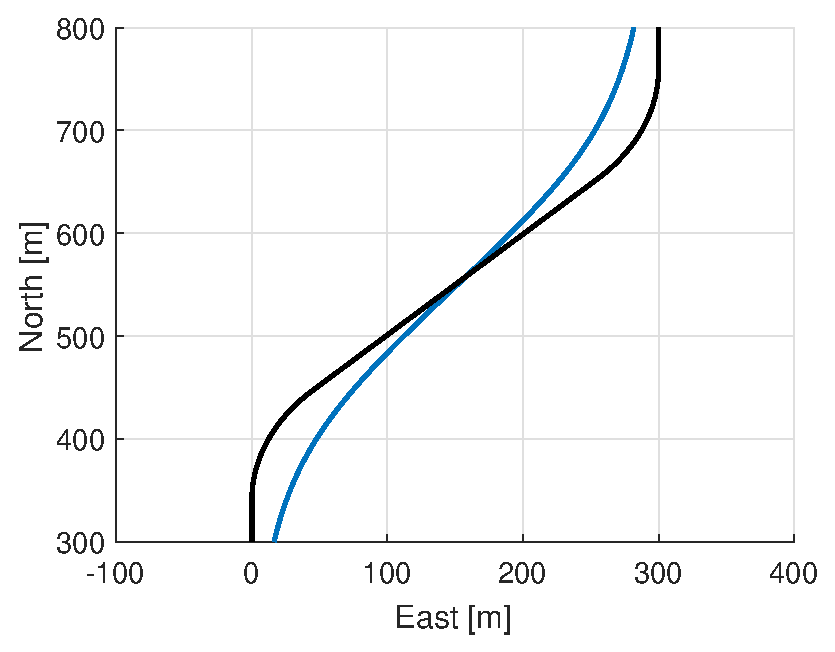
\includegraphics[width=0.5\textwidth, keepaspectratio=true]{../../results/opt/paths/fig_cur/uav_position_45deg_150m.eps}}
	\qquad
	\subfloat[UAV position $70\degree$]{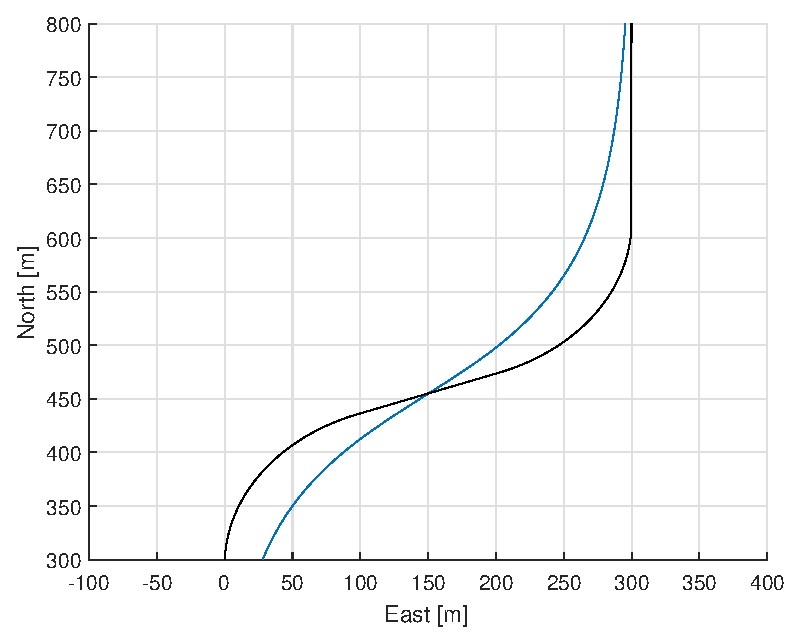
\includegraphics[width=0.5\textwidth, keepaspectratio=true]{../../results/opt/paths/fig_cur/uav_position_70deg_150m.eps}}}
	\makebox[\textwidth][c]{
	\subfloat[Camera position $45\degree$]{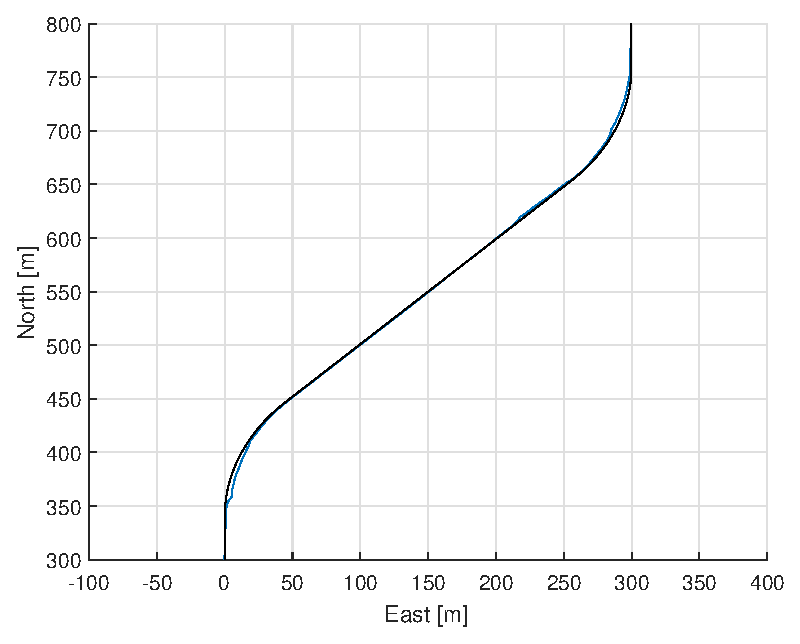
\includegraphics[width=0.5\textwidth, keepaspectratio=true]{../../results/opt/paths/fig_cur/camera_position_45deg_150m.eps}}
	\qquad
	\subfloat[Camera position $70\degree$]{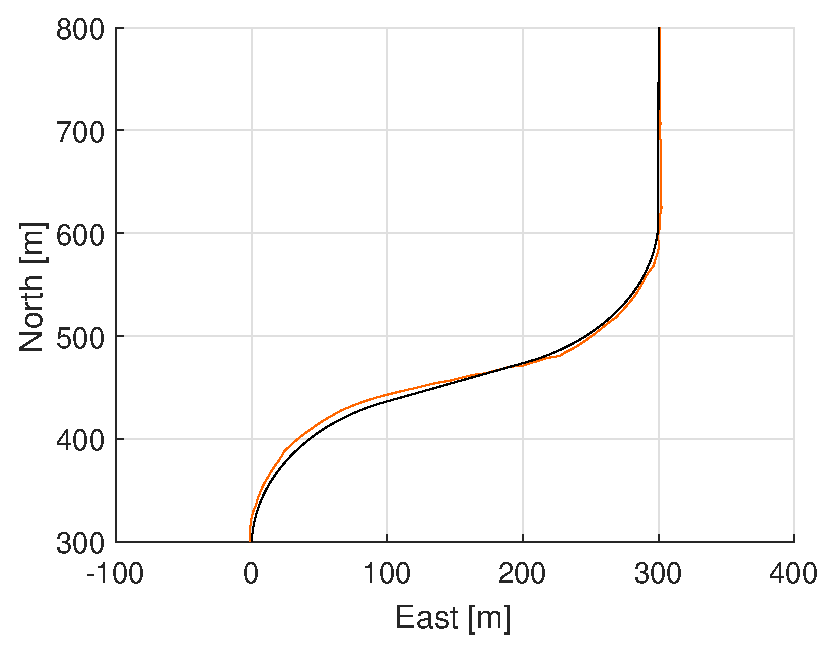
\includegraphics[width=0.5\textwidth, keepaspectratio=true]{../../results/opt/paths/fig_cur/camera_position_70deg_150m.eps}}}
	\makebox[\textwidth][c]{
	\subfloat[Heading angle]{\includegraphics[width=0.5\textwidth, keepaspectratio=true]{../../results/opt/paths/fig_cur/heading.eps}
	\label{fig:paths_cur_heading}}}
	\caption{UAV position, camera position and heading angle during two subsequent turns of $45\degree$ and $70\degree$.}
	\label{fig:paths_cur_150m}
\end{figure}


\subsection{Lawnmover Path}

The result of attempting to optimize a lawnmover-pattern path is shown in Figure \ref{fig:lawnmover}. The radius was set to be $250$m, as the optimization of $180\degree$ path show that the MPC performs well on this turn, and the line connecting to archs is set to $500$m.

\begin{figure}
	\makebox[\textwidth][c]{
	\subfloat[UAV position]{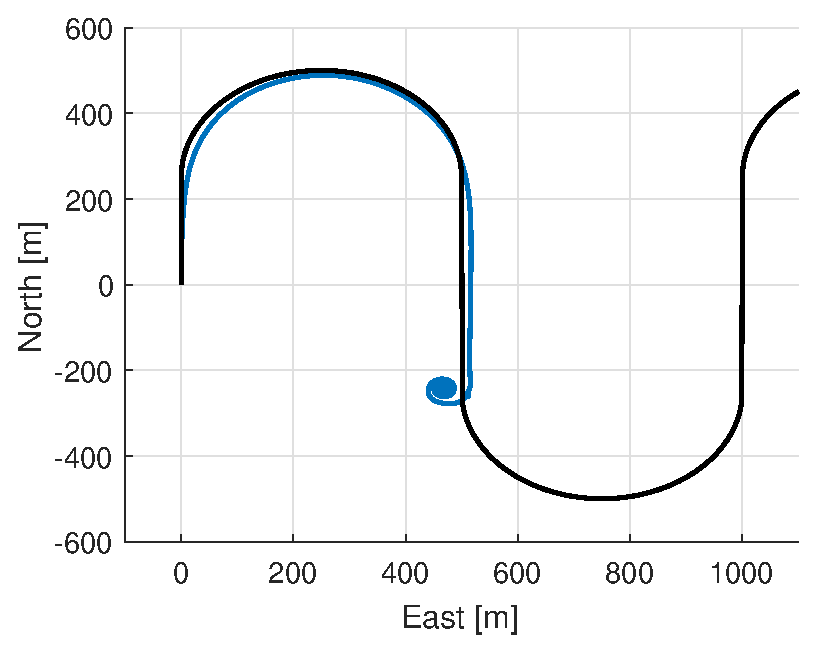
\includegraphics[width=0.5\textwidth, keepaspectratio=true]{../../results/opt/lawnmover/fig/uav_position.eps}}
	\qquad
	\subfloat[Camera position]{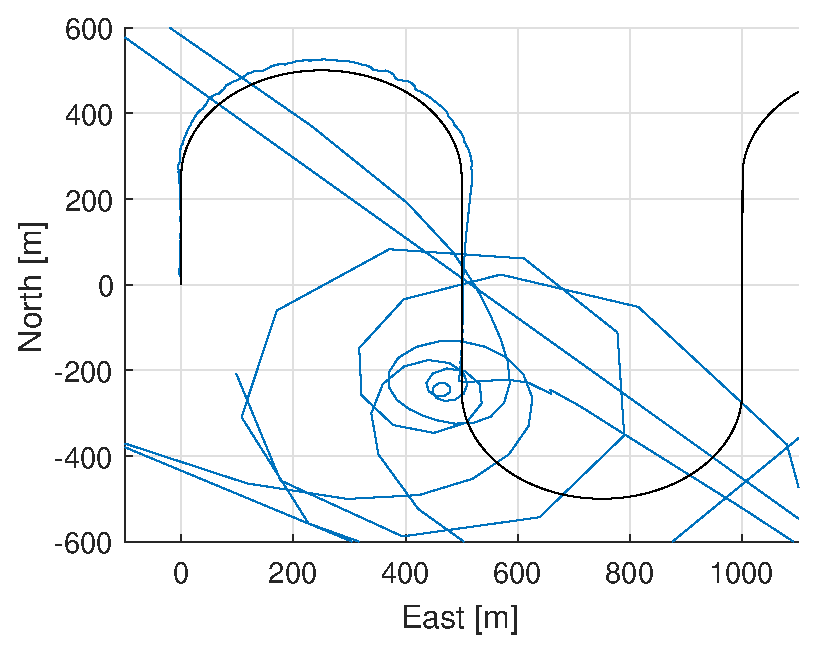
\includegraphics[width=0.5\textwidth, keepaspectratio=true]{../../results/opt/lawnmover/fig/camera_position.eps}}}
	\makebox[\textwidth][c]{
	\subfloat[Roll and pitch angle]{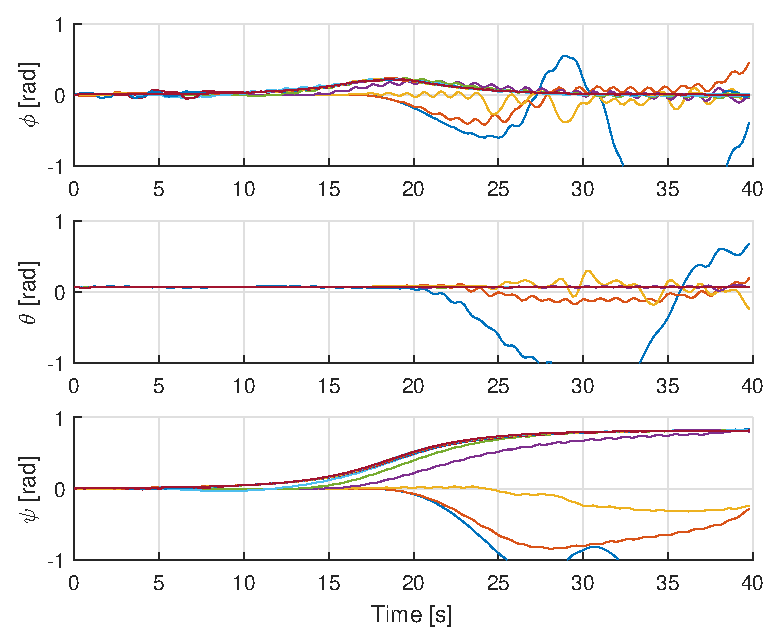
\includegraphics[width=0.5\textwidth, keepaspectratio=true]{../../results/opt/lawnmover/fig/attitude.eps}
	\label{fig:lawnmover_attitude}}}
	\caption{Result of attempting to optimize a lawnmover-pattern path with radius $250$m.}
	\label{fig:lawnmover}
\end{figure}

When the MPC optimizes the first $180\degree$ turn, it performs in a similar manner to the results in section \ref{subsec:180}: it takes the inner turn to begin with, and then widens the turn at the end in order to avoid changing the roll angle quickly. While it should have taken the advantage of the straight line to position the UAV right above the path so it could return to trimmed flight, it instead chooses continue flying next to the path with a constant roll angle to compensate for the offset from the path. It uses the rudder to compensate for the roll angle so it can travel at a constant course angle. The roll angle it uses to track the path while flying next to the path can be seen in Figure \ref{fig:lawnmover_attitude}.

As the UAV approaches the next $180\degree$ arch it is already on the inner side of the turn. However, instead of this being an advantage since it optimizes a $180\degree$ turn like this by taking the inner turn, it throws the UAV into an unstable right-turning spiral.